\documentclass[a4paper]{article}

\usepackage[english]{babel}
\usepackage[utf8]{inputenc}
\usepackage{amsmath}
\usepackage{graphicx}
\graphicspath{ {images/} }
\usepackage[colorinlistoftodos]{todonotes}

\title{Actividad 9}

\author{Jose Pablo Salazar Velazquez}

\date{abril de 2016}

\begin{document}
\maketitle

\section{Introducción}

El péndulo es un sistema físico que puede oscilar bajo la acción gravitatoria u otra característica física (elasticidad, por ejemplo) y que está configurado por una masa suspendida de un punto o de un eje horizontal fijos mediante un dispositivo que sirve para medir el tiempo.

Existen muy variados tipos de péndulos que, atendiendo a su configuración y usos, reciben los nombres apropiados: péndulo simple, péndulo compuesto, péndulo cicloidal, doble péndulo, péndulo de Foucault, péndulo de Newton, péndulo balístico, péndulo de torsión, péndulo esférico, etcétera.

Sus usos son muy variados: medida del tiempo (reloj de péndulo, metrónomo, ...), medida de la intensidad de la gravedad, etc.

El periodo de oscilación es independiente de la amplitud, al menos para pequeñas oscilaciones. En cambio, aquel depende de la longitud del hilo. El período de la oscilación de un péndulo simple restringido a oscilaciones de pequeña amplitud puede aproximarse por:
\begin{equation}
T \approx 2\pi \sqrt[]{\frac{l}{g}}
\end{equation}
Para oscilaciones mayores la relación exacta para el período no es constante con la amplitud e involucra integrales elípticas de primera especie:
\begin{equation}
T = 4\sqrt[]{\frac{l}{g}}K(\sin\frac{\varphi_0}{2}) = 4\sqrt[]{\frac{l}{g}}\int_{0}^{\frac{\pi}{2}}  \! \frac{d\theta}{\sqrt[]{1-\sin^2\frac{\varphi_0}{2}}} \
\end{equation}

Producto 1: Con la expresión anterior, reproduzca la figura que aparece al inicio de esta Actividad, que representa los errores relativos. T0 es la aproximación lineal, T2 a T10 representan la inclusion de 2 hasta 10 términos de la serie de potencias.
 
Producto 2: Finalmente, aplicando una serie de Maclaurin
\begin{equation}
\sin\frac{\theta_0}{2} = \frac{1}{2}\theta_0 - \frac{1}{48}\theta^3_0 + \frac{1}{3840}\theta^5_0 - \frac{1}{645120}\theta^7_0 + ...
\end{equation}


\section{Producto 1}
\subsection{Codigo}
\begin{verbatim}

from scipy.integrate import quad
import numpy as np
import matplotlib.pyplot as plt
import math

g=9.8        
l=2  


T0=2*np.pi*np.sqrt(l/g)
n=1000
e=0.0001
theta0=np.linspace(e,(np.pi)+e,n) 


#Definiendo arreglos para resultados arrojados
S=[0 for i in range(n)]
TT=[0 for i in range(n)]
R=[0 for i in range(n)]
T=[0 for i in range(n)]
real0=[0 for i in range(n)]
real2=[0 for i in range(n)]
real4=[0 for i in range(n)]
real6=[0 for i in range(n)]
real8=[0 for i in range(n)]

#------------------------------------------
#Creando doble loop para considerar los casos
#donde se agregan mas terminos de la serie de potencias


M0=0

#Comenzando un loop para poder calcular todos los resultados 
#posibles contemplando un angulo inicial variante
for i in range(M0):
    for j in range(0,n):
        F1=float(math.factorial(2*i))
        F2=float(((2**i)*(math.factorial(i)))**2)
        
        S[j]=np.sin(theta0[j]/2)**(2*i)
        TT[j]=((F1/F2)**2)*(S[j])
        R[j]=TT[j]+R[j]
        T[j]=R[j]*T0
        real0[j]=(T[j]/T0)
#------------------------------------------        
M2=2
for i in range(M2):
    for j in range(0,n):
        F1=float(math.factorial(2*i))
        F2=float(((2**i)*(math.factorial(i)))**2)
        
        S[j]=np.sin(theta0[j]/2)**(2*i)
        TT[j]=((F1/F2)**2)*(S[j])
        R[j]=TT[j]+R[j]
        T[j]=R[j]*T0
        real2[j]=(T[j]/T0)-1
#------------------------------------------        
M4=4
for i in range(M4):
    for j in range(0,n):
        F1=float(math.factorial(2*i))
        F2=float(((2**i)*(math.factorial(i)))**2)
        
        S[j]=np.sin(theta0[j]/2)**(2*i)
        TT[j]=((F1/F2)**2)*(S[j])
        R[j]=TT[j]+R[j]
        T[j]=R[j]*T0
        real4[j]=(T[j]/T0)-2
#------------------------------------------
M6=6
for i in range(M6):
    for j in range(0,n):
        F1=float(math.factorial(2*i))
        F2=float(((2**i)*(math.factorial(i)))**2)
        
        S[j]=np.sin(theta0[j]/2)**(2*i)
        TT[j]=((F1/F2)**2)*(S[j])
        R[j]=TT[j]+R[j]
        T[j]=R[j]*T0
        real6[j]=(T[j]/T0)-3
#------------------------------------------
M8=8
for i in range(M8):
    for j in range(0,n):
        F1=float(math.factorial(2*i))
        F2=float(((2**i)*(math.factorial(i)))**2)
        
        S[j]=np.sin(theta0[j]/2)**(2*i)
        TT[j]=((F1/F2)**2)*(S[j])
        R[j]=TT[j]+R[j]
        T[j]=R[j]*T0
        real8[j]=(T[j]/T0)-4

#Gráfica
plt.plot(theta0, real0, 'b',linewidth=2, label="T0")
plt.plot(theta0, real2, 'g',linewidth=2, label="T2")
plt.plot(theta0, real4, 'r',linewidth=2, label="T4")
plt.plot(theta0, real6, 'm',linewidth=2, label="T6")
plt.plot(theta0, real8, 'c',linewidth=2, label="T8")
plt.title('Error utilizando series de potencia')
plt.grid()
plt.xlabel('Angulo')
plt.xlim(0,np.pi)
plt.ylim(0,1)
plt.ylabel('Error')
plt.legend(loc='best')


fig = matplotlib.pyplot.gfc()
fig.set_size_inches(10.5,5.5)
fig.savefig('error.png',dpi=100)
\end{verbatim}
El error que arroja el programa, es el siguiente:
\linebreak
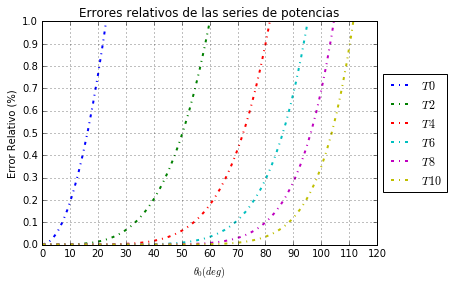
\includegraphics[width=9cm]{actividad_9} \\
\section{Serie de Mclaurin}
El resultado aproximado con serie de Mclaurin, fue el siguiente:
\linebreak
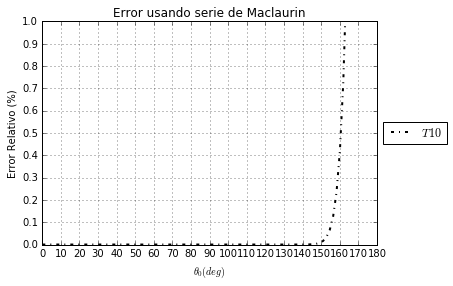
\includegraphics[width=9cm]{actividad_9-1}

\end{document}